\documentclass{beamer}
\usepackage[utf8]{inputenc}

\usetheme{Madrid}
\usecolortheme{default}
\usepackage{amsmath,amssymb,amsfonts,amsthm}
\usepackage{txfonts}
\usepackage{tkz-euclide}
\usepackage{listings}
\usepackage{adjustbox}
\usepackage{array}
\usepackage{tabularx}
\usepackage{gvv}
\usepackage{lmodern}
\usepackage{circuitikz}
\usepackage{tikz}
\usepackage{graphicx}
\usepackage{amsmath}

\setbeamertemplate{page number in head/foot}[totalframenumber]

\usepackage{tcolorbox}
\tcbuselibrary{minted,breakable,xparse,skins}



\definecolor{bg}{gray}{0.95}
\DeclareTCBListing{mintedbox}{O{}m!O{}}{%
  breakable=true,
  listing engine=minted,
  listing only,
  minted language=#2,
  minted style=default,
  minted options={%
    linenos,
    gobble=0,
    breaklines=true,
    breakafter=,,
    fontsize=\small,
    numbersep=8pt,
    #1},
  boxsep=0pt,
  left skip=0pt,
  right skip=0pt,
  left=25pt,
  right=0pt,
  top=3pt,
  bottom=3pt,
  arc=5pt,
  leftrule=0pt,
  rightrule=0pt,
  bottomrule=2pt,
  toprule=2pt,
  colback=bg,
  colframe=orange!70,
  enhanced,
  overlay={%
    \begin{tcbclipinterior}
    \fill[orange!20!white] (frame.south west) rectangle ([xshift=20pt]frame.north west);
    \end{tcbclipinterior}},
  #3,
}
\lstset{
    language=C,
    basicstyle=\ttfamily\small,
    keywordstyle=\color{blue},
    stringstyle=\color{orange},
    commentstyle=\color{green!60!black},
    numbers=left,
    numberstyle=\tiny\color{gray},
    breaklines=true,
    showstringspaces=false,
}


\title 
{2.10.10}
\date{September 09,2025}


\author 
{Abhiram Reddy-AI25BTECH11021}



\begin{document}


\frame{\titlepage}
%------------------------------------

% Question frame
\begin{frame}{Question}
Given that
\[
\mathbf{a} = \begin{pmatrix} 1 \\ 1 \\ 1 \end{pmatrix}, \quad
\mathbf{c} = \begin{pmatrix} 0 \\ 1 \\ -1 \end{pmatrix}, \quad
\mathbf{a} \cdot \mathbf{b} = 3, \quad
\mathbf{a} \times \mathbf{b} = \mathbf{c},
\]
find \(\mathbf{b}\).
\end{frame}

% Step 1
\begin{frame}{Solution - Step 1}
Express vectors as column matrices:
\[
\mathbf{a} = \begin{pmatrix} 1 \\ 1 \\ 1 \end{pmatrix}, \quad
\mathbf{b} = \begin{pmatrix} x \\ y \\ z \end{pmatrix}, \quad
\mathbf{c} = \begin{pmatrix} 0 \\ 1 \\ -1 \end{pmatrix}.
\]
\end{frame}

% Step 2
\begin{frame}{Solution - Step 2}
Use the dot product condition:
\[
\mathbf{a}^\top \mathbf{b} = x + y + z = 3.
\]

Use the cross product condition:
\[
\mathbf{a} \times \mathbf{b} = 
\begin{pmatrix}
z - y \\
x - z \\
y - x
\end{pmatrix}
= 
\begin{pmatrix}
0 \\
1 \\
-1
\end{pmatrix}.
\]

Which gives:
\[
\begin{cases}
z - y = 0, \\
x - z = 1, \\
y - x = -1.
\end{cases}
\]
\end{frame}

% Step 4
\begin{frame}{Solution - Step 3}
Solve the system:

From \(z - y = 0\):
\[
z = y.
\]

From \(y - x = -1\):
\[
y = x - 1.
\]

Substitute in \(x - z = 1\) (with \(z=y\)):
\[
x - y = 1 \implies x - (x - 1) = 1 \implies 1 = 1,
\]
which is consistent.
\end{frame}

% Step 5
\begin{frame}{Solution - Step 4}
Use the dot product:
\[
x + y + z = x + (x - 1) + (x - 1) = 3x - 2 = 3 \implies 3x = 5 \implies x = \frac{5}{3}.
\]

Then,
\[
y = \frac{2}{3}, \quad z = \frac{2}{3}.
\]


\textbf{Final Answer}
\[
\boxed{
\mathbf{b} = \begin{pmatrix} \frac{5}{3} \\[6pt] \frac{2}{3} \\[6pt] \frac{2}{3} \end{pmatrix}.
}
\]
\end{frame}

% C code frame 1
\begin{frame}[fragile]{C Code - Part 1}
\begin{verbatim}
#include <stdio.h>

int main() {
    // Given vectors a and c
    double a[3] = {1, 1, 1};
    double c[3] = {0, 1, -1};

    // Variables for b components
    double x, y, z;
\end{verbatim}
\end{frame}

% C code frame 2
\begin{frame}[fragile]{C Code - Part 2}
\begin{verbatim}
    // From the solution:
    // z = y
    // y = x - 1
    // x + y + z = 3  =>  x + (x-1) + (x-1) = 3  => 3x - 2 = 3  => x = 5/3

    x = 5.0 / 3.0;
    y = x - 1.0;
    z = y;

    // Print result
    printf("Vector b is:\n");
    printf("b = [%.6f, %.6f, %.6f]\n", x, y, z);

    return 0;
}
\end{verbatim}
\end{frame}

% Python code frame 1
\begin{frame}[fragile]{Python Code - Part 1}
\begin{verbatim}
import numpy as np
import matplotlib.pyplot as plt
from mpl_toolkits.mplot3d import Axes3D

# Define the vectors
a = np.array([1, 1, 1])
b = np.array([5/3, 2/3, 2/3])
c = np.array([0, 1, -1])

origin = np.array([0, 0, 0])

fig = plt.figure()
ax = fig.add_subplot(111, projection='3d')
\end{verbatim}
\end{frame}

% Python code frame 2
\begin{frame}[fragile]{Python Code - Part 2}
\begin{verbatim}
# Plot vectors a, b, and c
ax.quiver(*origin, *a, color='r', label='a', arrow_length_ratio=0.1)
ax.quiver(*origin, *b, color='g', label='b', arrow_length_ratio=0.1)
ax.quiver(*origin, *c, color='b', label='c', arrow_length_ratio=0.1)

ax.set_xlim([0, 2])
ax.set_ylim([0, 2])
ax.set_zlim([-2, 2])

ax.set_xlabel('X')
ax.set_ylabel('Y')
ax.set_zlabel('Z')

ax.legend()
ax.set_title('Vectors a, b, and c in 3D')

plt.savefig('python_plot.png')
# plt.show()
\end{verbatim}
\end{frame}




\begin{frame}{Plot}
    \centering
    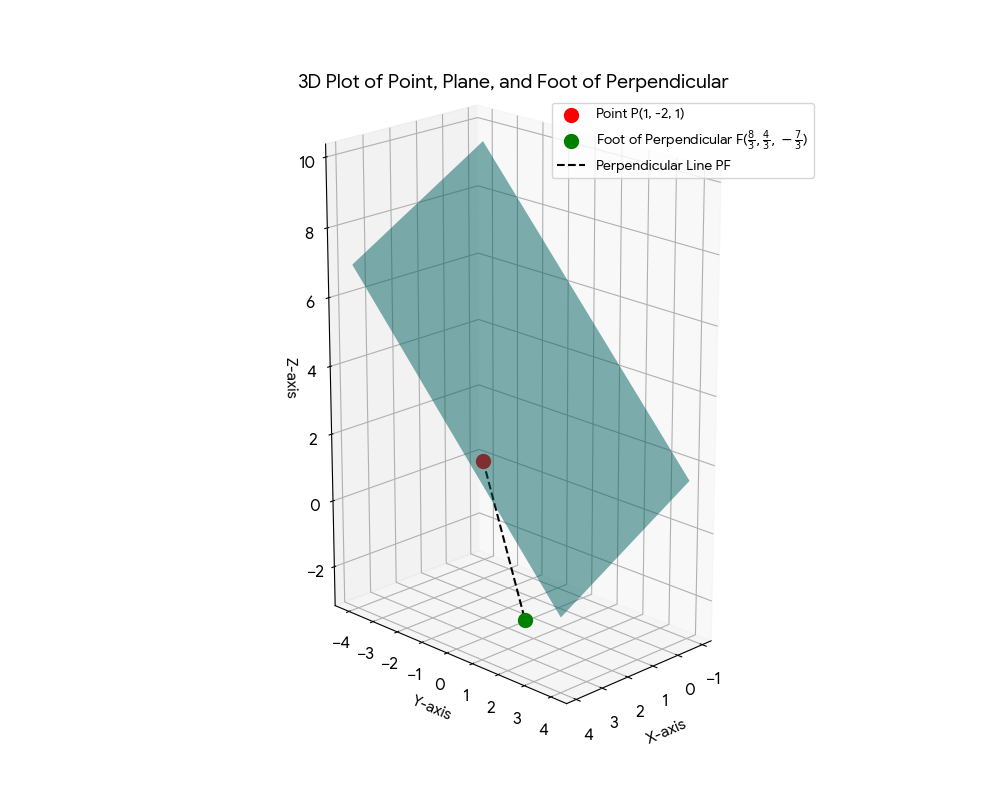
\includegraphics[width=\columnwidth, height=0.8\textheight, keepaspectratio]{figs/python_plot.png}     
\end{frame}


\end{document}